\section{Prediction of occultations} \label{Sec: predictions}

The prediction of the occultations was made by crossing the stellar coordinates and proper motions of the UCAC4 catalogue \citep{Zacharias2013} with the ephemeris presented in Sec. \ref{Sec: integration}. The search for stellar candidates follows the same procedure as presented by \cite{Assafin2010, Assafin2012} and \cite{Camargo2014}.

We predicted occultations for the 8 major irregular satellites of Jupiter,  Ananke, Carme, Elara, Himalia, Leda, Lysithea, Pasiphae and Sinope, and for Phoebe of Saturn and Triton and Nereid of Neptune.

For Triton and Nereid, the candidates for stellar occultations in 2016 were searched using the WFI catalogue in the same way as the predictions for Centaurs and TNOs occultations by \cite{Assafin2010, Assafin2012} and \cite{Camargo2014}. This catalogue contains the stars in the path of Neptune in the sky up to mid-2016. The catalogue was generated by observations made at the ESO 2p2 telescope (IAU code 809) using the Wide Field Imager (WFI) CCD mosaic detector. The filter used was the broad-band R filter ESO\#844 with $\lambda_c$ = 651.725 nm and $\Delta\lambda$ = 162.184 nm.

A total of 396 events were identified between January 2016 and December 2017. In Table \ref{Tab: satellite-occultation} we present the number of stellar occultations predicted by year for each satellite. Table \ref{Tab: occ-list} shows a sample of the catalogue of occultations generated and their parameters, which are necessary to produce occultation maps. Since these objects are very small, the duration of each event is a few seconds. All the occultation tables and maps will be publicly available at the CDS. No star brighter than MagR*=18 will be occulted by Triton in 2016. For this satellite, we cut events with stars fainter than R=18, since for Triton the flux drop during such an occultation would be very small. In Fig. \ref{Fig: ocultacao} we show an example of an occultation map. This is the only found occultation by Triton and it will happen in October 05, 2017. This event can be observed from Europe and the east coast of USA and will be a great opportunity to study in high resolution the atmosphere of the satellite.

\begin{table}
\caption{\label{Tab: satellite-occultation} Number of stellar occultations for each satellite from January, 2016 up to December, 2017.}
\begin{centering}
\begin{tabular}{lccc}
\hline  \hline
%\multicolumn{4}{c}{Diameter of the satellites} \tabularnewline
Satellite  & 2016 & 2017 & Total \tabularnewline
\hline
Ananke & 12 & 16 & 28 \tabularnewline
Carme & 20 & 14 & 34 \tabularnewline
Elara & 14 & 16 & 30 \tabularnewline
Himalia & 15 & 12 & 27 \tabularnewline
Leda & 8 & 24 & 32 \tabularnewline
Lysithea & 16 & 11 & 27 \tabularnewline
Pasiphae & 20 & 19 & 39 \tabularnewline
Sinope & 15 & 21 & 36 \tabularnewline
\hdashline
Phoebe\tablefootmark{a} & 32 & 98 & 130 \tabularnewline
\hdashline
Nereid\tablefootmark{a} & 11\tablefootmark{b} & 1 & 12 \tabularnewline
Triton\tablefootmark{a} & -- & 1 & 1 \tabularnewline
\hline
\end{tabular}
\par \end{centering}
Occultations predicted using the UCAC4 catalogue and STE ephemeris.
\tablefoottext{a}{Using JPL ephemeris.}
\tablefoottext{b} {Using the WFI catalogue as explained in Sec. \ref{Sec: predictions}}.
\end{table}

\begin{table*}
\caption{\label{Tab: sample-cds} A sample of stellar occultation predictions for Pasiphae}
\begin{centering}
\begin{tabular}{cccrcccrcrr}
\hline
\hline
d m Year~~~~h~~m~~~s & RA~~~(ICRS)~~~Dec & C/A & P/A & $\nu$ & {\it D} & $R^*$ & $\lambda$ & LST & $\mu_{\alpha*}$ & $\mu_{\delta}$ \tabularnewline
\hline
% & \multicolumn{2}{c}{Mean errors} & Nr & Nr &  UCAC4       \tabularnewline
09 04 2016 03:58:19. & 11 14 36.7707 +07 39 20.7610 & 1.003 &  17.9 & -12.88 &  4.54 & 14.9 & 271. & 22:03 &  12. & -33. \tabularnewline 
13 06 2016 00:16:12. & 11 12 48.5020 +07 06 43.3520 & 0.661 &  30.0 & +14.32 &  5.50 & 13.9 & 262. & 17:45 &  -1. &   1. \tabularnewline 
27 06 2016 13:56:09. & 11 18 03.4160 +06 23 45.1940 & 1.707 &  28.0 & +20.29 &  5.74 & 11.7 &  44. & 16:53 &   4. & -10. \tabularnewline 
18 07 2016 15:07:24. & 11 28 15.5076 +05 05 31.8060 & 0.942 &  26.7 & +27.80 &  6.05 & 14.0 &   8. & 15:40 &   4. &   4. \tabularnewline 
22 07 2016 16:15:07. & 11 30 30.4310 +04 48 43.4340 & 0.644 & 206.5 & +29.04 &  6.11 & 14.6 & 348. & 15:27 &  23. & -24. \tabularnewline 
24 07 2016 01:37:34. & 11 31 17.8471 +04 42 49.0540 & 0.029 & 206.6 & +29.46 &  6.12 & 15.1 & 206. & 15:22 &   2. &  -8. \tabularnewline 
24 07 2016 17:37:18. & 11 31 40.7472 +04 39 57.5060 & 0.840 &  26.5 & +29.66 &  6.13 & 14.9 & 326. & 15:20 & -11. &  -1. \tabularnewline 
\hline
\end{tabular}
\par\end{centering}
\textbf{Notes}. Entries included: day of the year and UTC time of the prediction; right ascension and declination of the occulted star - at the central instant of occultation (corrected by proper motions); C/A: the geocentric closest approach, in arcseconds; P/A: the satellite position angle with respect to the occulted star at C/A, in degrees (zero at north of the star, increasing clockwise); $\nu$: velocity in the plane of sky, in km s$^{-1}$: positive = prograde, negative = retrograde; {\it D}: planet range to Earth, in AU; $R^*$: normalized magnitude to a common shadow velocity of 20 km s$^{-1}$ by the relationship $\textrm{R}^* = \textrm{R}_{\textrm{actual}} + 2.5 \times \log 10 \left(\frac{\textrm{velocity}} {20 \textrm{km}\, \textrm{s}^{-1}} \right)$; $\lambda$: east longitude of subplanet point in degrees, positive towards east; LST: UT + $\lambda$: local solar time at subplanet point, hh:mm; $\mu_{\alpha *}$ and $\mu_{\delta}$: proper motions in right ascension and declination, respectively (mas/year).
\label{Tab: occ-list}
\end{table*}

\begin{figure*}
\begin{centering}
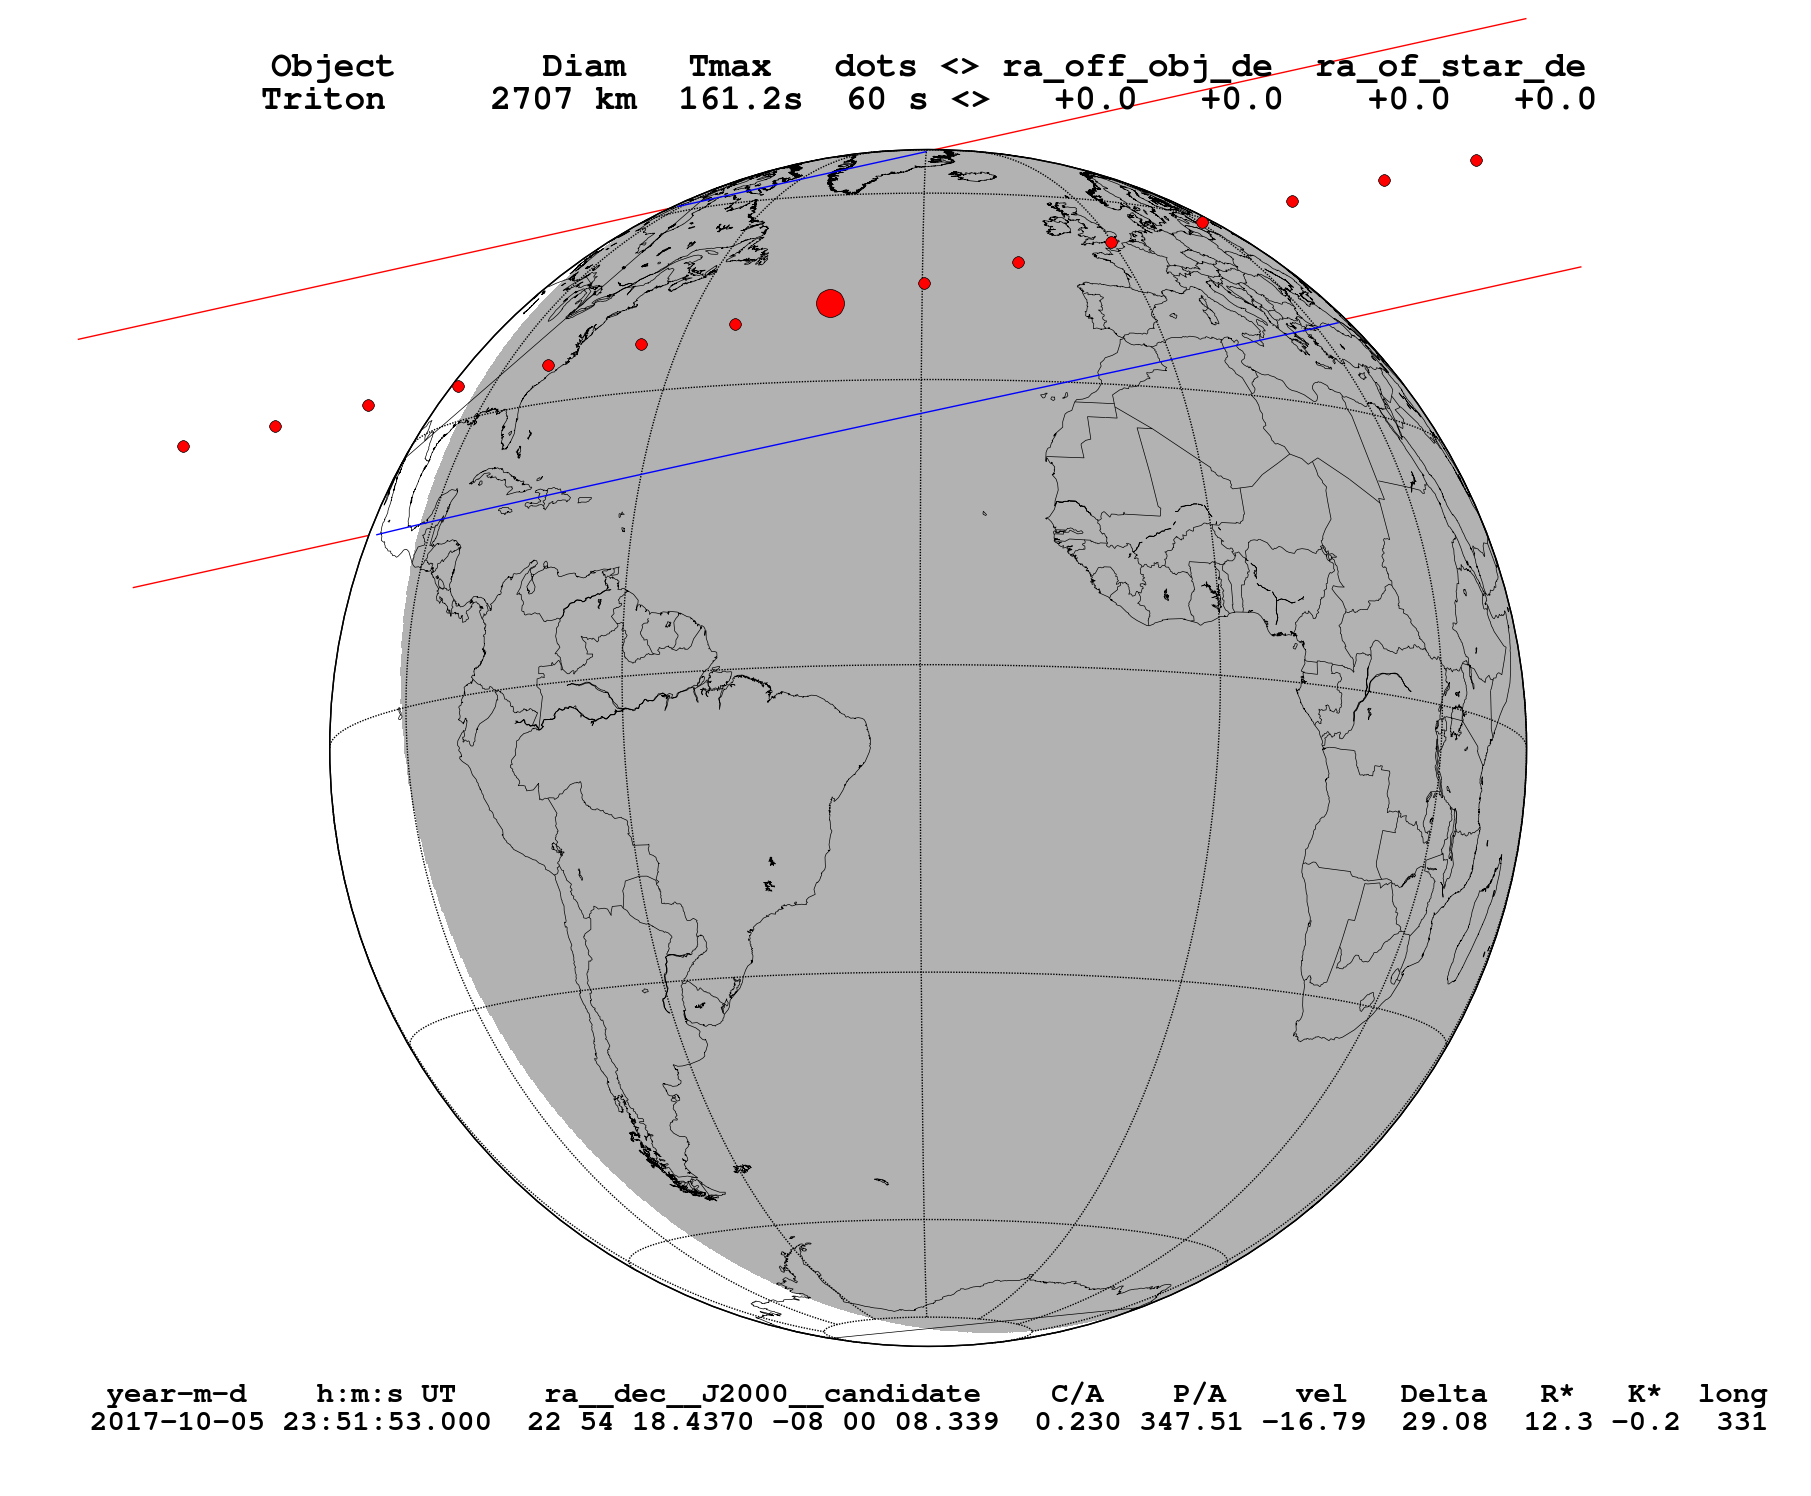
\includegraphics[scale=0.4]{figures/Triton_2017-10-05T23:51:53.png}   
\caption{Occultation map for Triton.% regarding to the first event sampled in Table \ref{Tab: occ-list}.
The central red dot show the geocentric closest approach of the shadow. The small ones shows the center of the shadow separated by 60s. The lines show the path of the shadow over the Earth. The shadow moves from right to left.
\textbf{Labels:} Diam: Diameter of the object; Tmax: Maximum duration of the event for a central observation; C/A: the geocentric closest approach, in arcseconds; P/A: the satellite position angle with respect to the occulted star at C/A, in degrees; vel: velocity of event in km/s; Delta: Geocentric distance to the occulting object in AU; $R^*$: normalized magnitude to a common shadow velocity of 20 km s$^{-1}$; long: east longitude of subplanet point in degrees, positive towards east.}
\label{Fig: ocultacao}
\end{centering}
\end{figure*}

The first preliminary catalogue version of the ESA astrometry satellite GAIA \citep{deBruijne2012} is expected to be released up to the end of 2016. The precise star positions to be derived by GAIA will provide better predictions with the main source of error being the ephemeris. Astrometric reduction of observations published in \cite{GomesJunior2015} will be revised with the GAIA catalogue and the predictions from 2017 onwards will be improved. Since we cannot foresee exactly when the GAIA catalogue will be released and when new and re-reduced satellite positions in the GAIA frame will become available, we decided to publish only the predictions for occultations restricted to the 2016-2017 time interval.


\section{Occultation test} \label{Sec: testes}

Observing a stellar occultation demands a great effort. And, in our case, the shadow covers a very restricted area on Earth because of the size of the irregular satellites. Since no stellar occultation by an irregular satellite was observed up to date, with the exception of Triton, and since we want to be sure that we can start observational campaigns with reasonable chances of success, we tested an occultation prediction for a large target, to assess the quality of the prediction.

The test design consisted in observing the object and star to be occulted near the date of the event predicted when the two objects were present in the same field of view (FOV), close to each other. Thus, the relative positions between the two objects had minimal influence of the errors of the reference catalogue of stars used and possible field distortions \citep[and references therein]{Peng2008}. The relative positions of the star and satellite were used to check the original predictions. Notice that in the test we do not attempt to observe any actual occultation. The test could be performed at any site, regardless of the Earth location where the occultation would in fact be visible. 

We tested the occultation by Himalia predicted to occur on March 3, 2015. The shadow would cross the northern part of South America. For the event, four situations were considered:
\begin{enumerate}[I]
\item Our nominal, published prediction with the STE ephemeris (see Sec. \ref{Sec: integration}), and the nominal UCAC4 position of the star;
\item Prediction with the JPL ephemeris and the nominal UCAC4 position of the star;
\item From star and satellite offsets calculated from observations made a few days before the occultation when the objects were very separated (different FOVs);
\item Same as 3 but with the star and the satellite close in the same FOV.
\end{enumerate}

Table \ref{Tab: comparison-Himalia} shows the differences between the predictions in the four situations. For situation 3 we observed the objects on February 22 with the Zeiss telescope (diameter = 0.6m; FOV = $12\farcm6$; pixel scale = $0\farcs37 / pixel$) at the Observatório do Pico dos Dias, Brazil (OPD, IAU code 874, 45\degr 34\arcmin 57\arcsec W, 22\degr 32\arcmin 04\arcsec S, 1864m). On that day, Himalia and the star were observed in separate FOVs as they were still far apart. On the night of the event, March 3, the objects were observed with Perkin-Elmer telescope (diameter = 1.6m; FOV = $5\farcm8$; pixel scale = $0\farcs17 / pixel$) at OPD just over an hour after the time scheduled for the event. Satellite and star were separated by about 16 arcsec, so very close to each other (situation 4). From the calculated offsets, the center of the shadow was obtained. Notice that the shadow path was not predicted to cross the OPD (which was located at almost 2000 km south from the shadow path). This was not necessary for testing the prediction.

%\begin{figure*}
%\begin{centering}
%\subfigure[Prediction with STE ephemeris]{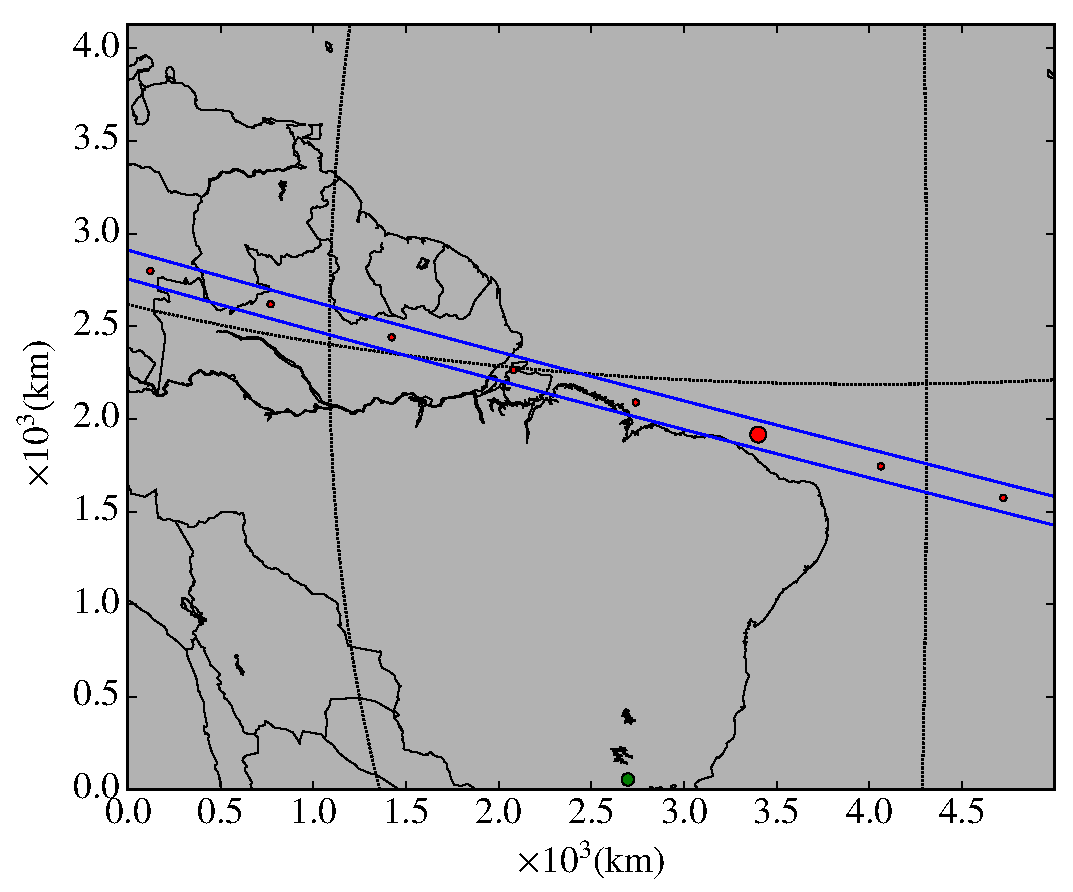
\includegraphics[width=8.8cm]{figures/Himalia_STE.eps}  \label{Fig: occ-Himalia-STE}}
%\subfigure[Prediction with JPL ephemeris]{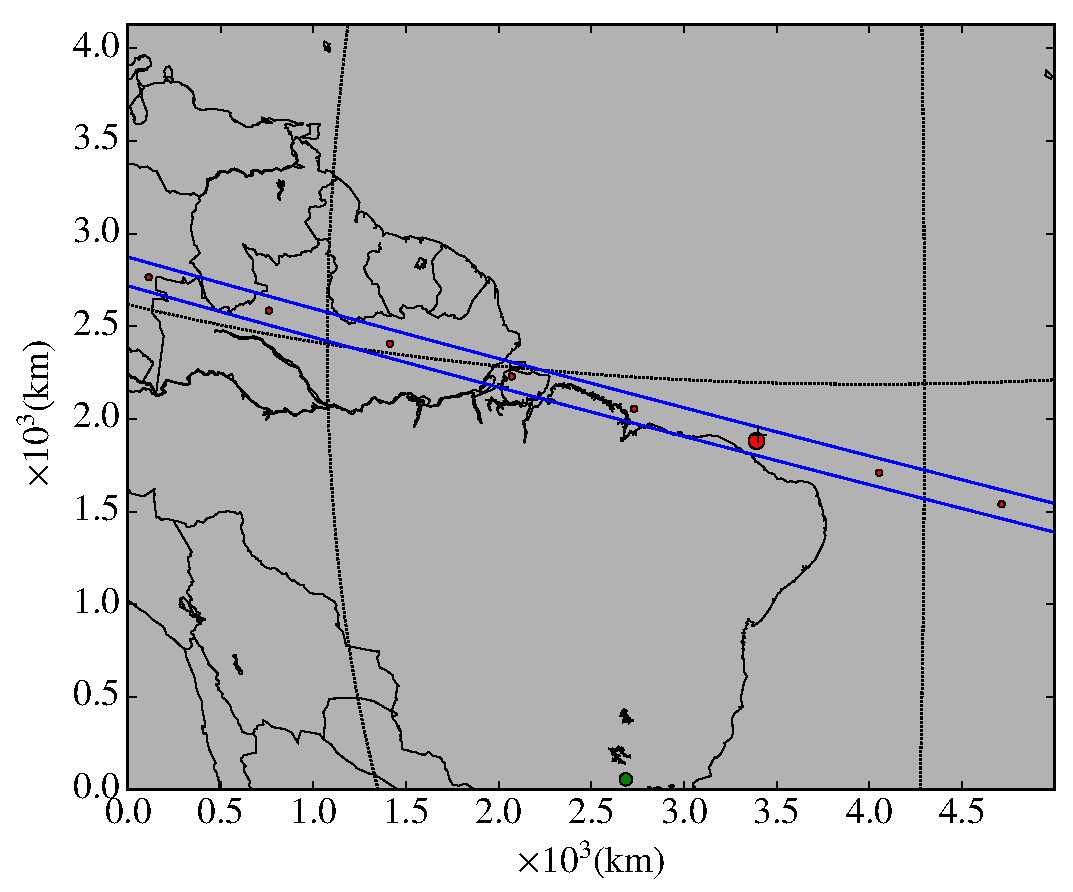
\includegraphics[width=8.8cm]{figures/Himalia_JPL.eps}  \label{Fig: occ-Himalia-JPL}}
%\subfigure[Observation at February 22 (different FOVs)]{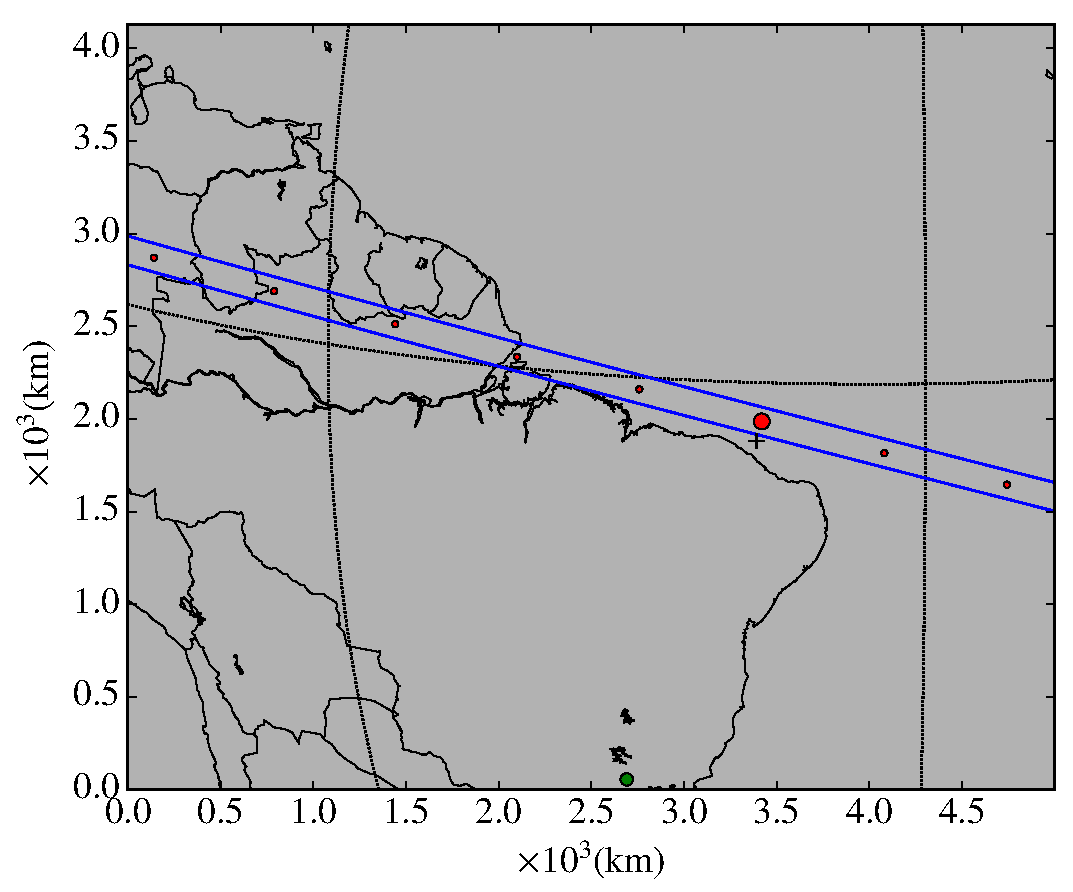
\includegraphics[width=8.8cm]{figures/Himalia_22fev.eps}   \label{Fig: occ-Himalia-off22fev}}
%\subfigure[Observation at March 03 (same FOV)]{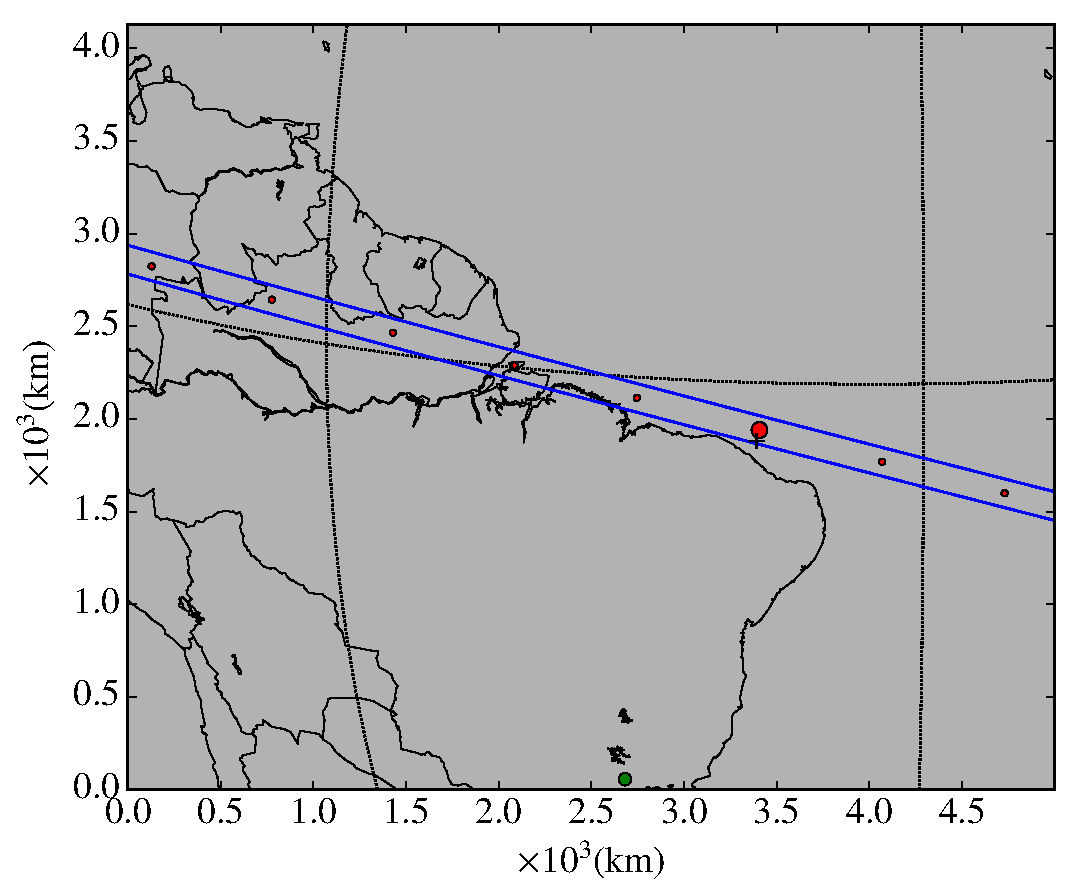
\includegraphics[width=8.8cm]{figures/Himalia_03mar.eps}   \label{Fig: occ-Himalia-off03mar}}
%\caption{Predictions for Himalia: The straight lines show the size of the shadow. The big red dot show the geocentric closest approach of the shadow. The black "+" marks at maps (b,c,d) are the STE prediction closest approach for reference. The small red ones are the center of the shadow separated by one minute. \ref{Fig: occ-Himalia-STE} is the map using the STE ephemeris showed in Sec. \ref{Sec: integration}. \ref{Fig: occ-Himalia-JPL} shows the shadow using the JPL ephemeris. In \ref{Fig: occ-Himalia-off22fev} we apply offsets to the positions of star and satellite accordingly the observations made at February 22. \ref{Fig: occ-Himalia-off03mar} is as in \ref{Fig: occ-Himalia-off22fev} but with observations made at March 03 when the objects were close to each other. The green dot at the bottom of the maps is the location of Observatório do Pico dos Dias.}
%\label{Fig: occ-Himalia}
%\end{centering}
%\end{figure*}

%\begin{figure*}
%\begin{centering}
%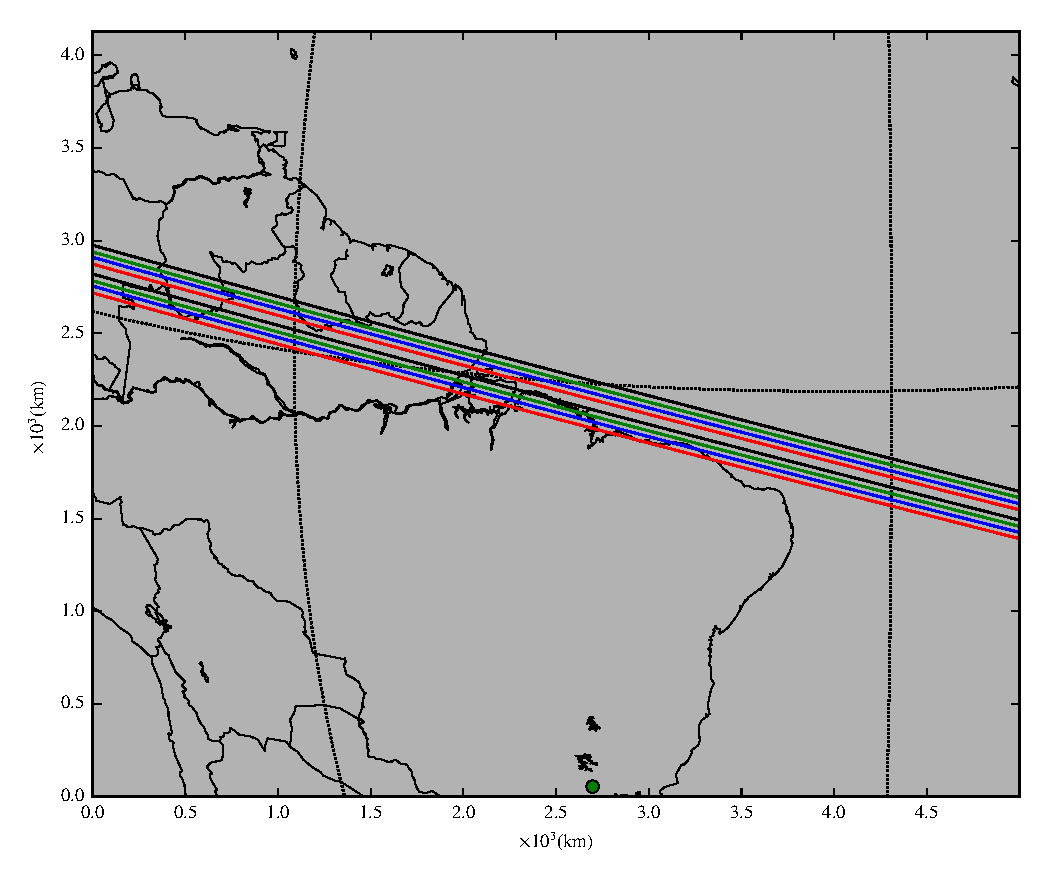
\includegraphics[width=17.6cm]{figures/HIMALIA.eps}
%\caption{Predictions for Himalia: The straight lines show the center of the shadow over time. In blue is for the prediction using the STE ephemeris showed in Sec. \ref{Sec: integration}. In red the shadow using the JPL ephemeris. In black we apply offsets to the positions of star and satellite accordingly the observations made at February 22. In green, the same for the previous one but with observations made at March 03 when the objects were close to each other. The dots show the closest approach of the shadow for each prediction. The scales are relative to the closest approach of the prediction using the STE ephemeris. The bars show the estimated diameter of the satellite and estimated error of the prediction.}
%\label{Fig: occ-Himalia}
%\end{centering}
%\end{figure*}

The critical parameter in the comparisons is the C/A, which here is related to latitudes. The apparent radius of Himalia is about 20 mas (see Table 1). In the context of the test, for a 0 mas offset in C/A we would have 100\% probability of observing the occultation, and 0\% in the case of a C/A offset equal to or larger than 20 mas, the radius of Himalia. From Table 5, we have nearly 0\% probability of success in situation 3, for which the offset in C/A was -20 mas, but when the relative astrometry was poor, 10 days prior to the event. Once at the day of the event in situation 4, the C/A offset dropped to -9 mas only, corresponding to a 55\% probability of success. Comparison with the prediction using the JPL ephemeris (situation 2) gives a +11 mas C/A offset, or a compatibility of 45\% between the ephemerides. All this suggests that there was a good probability of observing the event. The largest differences between the shadows of the four situations were 36s in time along the shadow path and 101km (31 mas) in the direction perpendicular to the shadows, suggesting that observers should be spread in narrow latitude ranges 100 km wide.

\begin{table}
\caption{\label{Tab: comparison-Himalia} Comparison between the predictions of the Himalia occultation at March 03, 2015.}
\begin{centering}
\begin{tabular}{lccc}
\hline  \hline
\multicolumn{4}{c}{Differences with respect to the STE prediction} \tabularnewline
Method  & Instant of C/A  & C/A & Sit.   \tabularnewline
\hline
STE & 00:39:51 UTC & $0\farcs703$ & I \tabularnewline
JPL & -26s & +11mas (36km) & II \tabularnewline % (284km)
Feb. 22 Obs. & -14s & -20mas (65km) & III \tabularnewline % (153km)
Mar. 03 Obs. & -36s & -09mas (29km) & IV \tabularnewline % (393km)
\hline
\end{tabular}
\par\end{centering}
C/A: geocentric closest approach; Sit: Situation test considered.
\end{table}

%The second test was with the satellite Elara, which is the second largest irregular satellite of Jupiter. The event was predicted to occur at March 30, 2015. The observations were made on March 25 and April 2, 2015 with the Zeiss telescope. On the night of April 2 the star and satellite could still be observed in the same FOV. Due to Elara being fainter than Himalia by 2 magnitudes, dispersions of the satellite positions on both nights ended up being higher than for Himalia. %Still, the differences between the maps obtained were relatively small. 
%The largest differences between them were 144s (186 mas) in time along the shadow path and 525 km (153 mas) perpendicular to it (see table \ref{Tab: comparison-Elara}).

%\begin{table}
%\caption{\label{Tab: comparison-Elara} Comparison between the predictions of Elara occultation at March 30, 2015.}
%\begin{centering}
%\begin{tabular}{lcc}
%\hline  \hline
%\multicolumn{3}{c}{Difference from STE prediction} \tabularnewline
%Method  & Instant of C/A  & C/A  \tabularnewline
%\hline
%STE & 01:45:13 UTC & $1\farcs082$ \tabularnewline
%JPL & +02s & +57mas(195km) \tabularnewline
%Mar. 25 Obs. & -70s & +20mas (68km) \tabularnewline
%Apr. 02 Obs. & +74s & -96mas (330km) \tabularnewline
%\hline
%\end{tabular}
%\par\end{centering}
%\end{table}